\section{Introduction}
\label{chapter:Introduction}

% \textbf{Big Picture.}
The object-oriented programming (OOP) paradigm and the C++ programming language are the de facto standard for developing large, complex and efficient software systems, in particular, 
when runtime performance and reliability are primary objectives.

A key building block of (runtime) OOP polymorphism are virtual functions, which enable late binding and allow programmers to overwrite a virtual function of the base-class with their 
own implementations. In order to implement virtual functions, the compiler needs to generate a virtual table meta-data structure of all virtual functions for each class containing 
them and provide to each instance of such a class a (virtual) pointer to the aforementioned table. While this approach allows for more flexible code to be built, 
the basic implementation provides unfortunately very little security assurances. Data about highly damaging arbitrary code executions in major applications collected by U.S. NIST 
(see Figure~\ref{ace:nvd:statistics}~\footnote{Number (\#, left Fig.) and percentage (\%, right Fig.) of arbitrary code executions (ACE) reports related (all colors expect black) to pointer or virtual table (vptr/vtbl) corruption 
(see bag of words at the bottom of left Fig.)* reported by U.S. NVD for the past 10 years~\cite{NVD:ACE}. In black are the ACE unrelated reports.
X axis is years (left \& right) and Y axis is number of reports in logarithmic scale (left) and distribution in \% of the same reports (right).
As of May'17, NVD reports in total 701 ACEs from which 143 are the result of a vptr/vtable corruption (see * above) that are exploited by highjacking forward indirect calls.
These vulnerabilities were reported in applications such as Google's Chrome \& V8 JavaScript engine, Mozilla Firefox, Microsoft's IE 10, Edge \& Chakra JavaScript engine, and several iOS/MacOS applications.} 
and~\cite{NVD:ACE}) demonstrates the security shortcomings and the need to address this problem space.


\begin{figure}[t!]
\centering
\hspace{-.24cm}
  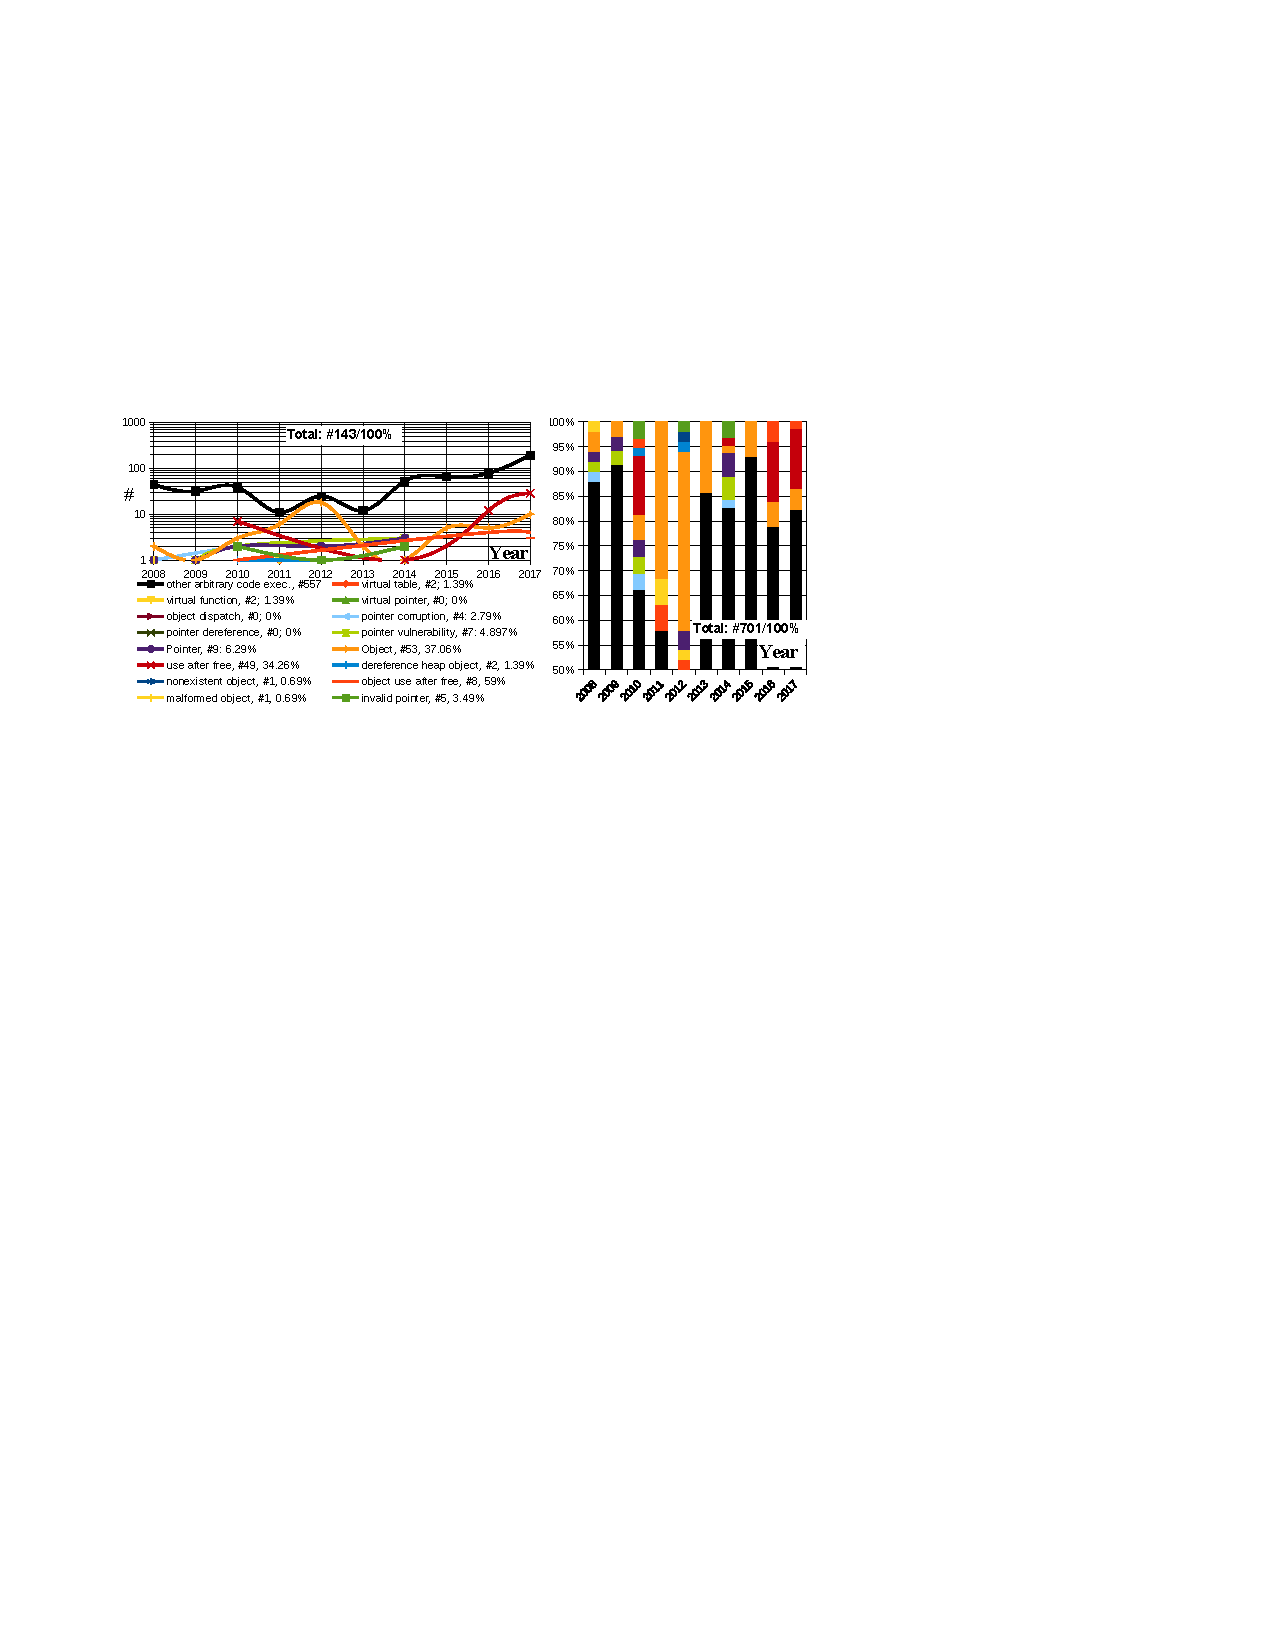
\includegraphics[scale=0.74]{figures/distri.pdf}
%   \node[below=of img, node distance=0cm, yshift=1.2cm, xshift=.25cm, font=\color{black}] {Year};
%   \node[left=of img, node distance=0cm, rotate=90, anchor=center,yshift=-.9cm,font=\color{black}] {\# Bad Type Casts Reported};
% \vspace{-.73cm}
\caption{10 Years of Arbitrary Code Reuse Attacks Statistics.}
\label{ace:nvd:statistics}
\vspace{-.5cm}
\end{figure}

While the reasons for unwanted outcomes can be highly diverse, our work is primarily motivated by memory corruption attacks (\textit{e.g.,} buffer/integer overflows), which can enable the 
execution of sophisticated Code-Reuse Attacks (CRAs) such as the advanced COOP attack~\cite{schuster:coop} and its 
extensions~\cite{crane:readactor++, subversive-c:lettner, ctf:coop, loop:oriented}. A necessary ingredient for this class of attacks is the ability
to corrupt the virtual pointer of an object.

To address such object dispatch corruptions, Control-Flow Integrity (CFI)~\cite{abadi:cfi2, abadi:cfi} was originally developed to secure indirect control flow transfers by adding 
runtime checks before each indirect callsite. Unfortunately, COOP and its brethren bypass most deployed CFI-based enforcement policies, since these attacks do not exploit indirect 
backward edges (\textit{i.e.,} return edges), but rather exploit the forward indirect control flow transfer imprecision which cannot be determined statically upfront as alias analysis is 
undecidable~\cite{alias:undecidable} in program binaries.

More recent techniques and tools can be distinguished into those relying on \textit{source code} access including SafeDispatch~\cite{safedispatch:jang}, ShrinkWrap~\cite{haller:shrinkwrap}, 
VTI~\cite{bounov:interleaving}, and IFCC/VTV~\cite{vtv:tice}; the latter being used in production, but the reliance on source-code availability limits the applicability of the approach. 
In contrast, \textit{binary}-based tools typically rely on forward-edge CFI policies. Examples include binCFI~\cite{ccfir:zhang, zhang:usenix}, VCI~\cite{vci:asiaccs} and 
TypeArmor~\cite{veen:typearmor}. 

According to our assessment of the literature, TypeArmor serves as the state-of-the-art of binary-based defense tools against advanced CRAs. In TypeArmor, a fine-grained 
forward edge CFI-policy based on parameter count for binaries is implemented. It calculates invariants for calltargets and indirect callsites based on the number of parameters they use 
by leveraging static analysis of the binary, which then is patched to enforce those invariants during runtime. While we believe the general approach to be highly promising, we consider 
as a significant shortcoming that TypeArmor lacks precision with respect to the number of calltargets allowed per callsite which introduces significant 
inefficiencies (see~\cref{{Too Permissive Parameter-Based Policies}} for more details). 
% With our work, we aim to achieve both significant precision and efficiency enhancements.

In this paper, we present \textsc{TypeShield}, a runtime binary-level filtering tool for illegitimate forward calls, that is based on an improved forward-edge fine-grained CFI-policy 
compared to previous work~\cite{veen:typearmor}. 
\textsc{TypeShield} takes the binary of a program as input and it automatically instruments it in order
to detect illegitimate indirect calls at runtime. In order to achieve this, 
\textsc{TypeShield} analyzes 64-bit binaries by focusing on function parameters which are passed with the 
help of registers. Based on the used ABI, \textsc{TypeShield} is consequently able to track 4 or 6 arguments for the Microsoft's x64-bit calling convention or System V ABI, 
respectively. Similarly to TypeArmor, we do not take into consideration floating-point arguments passed via xmm registers; which we want to address in future work. 
As we demonstrate in the evaluation section, this setup provides us with enough information to be significantly more precise than~\cite{veen:typearmor} when aiming to stop several state-of-the-art CRAs.



%% \textbf{Problem.}
%The performance benefit of late binding comes with high security implications (\textit{i.e.,} arbitrary code executions~\cite{NVD:ACE} reported by NIST NVD, see Figure~\ref{ace:nvd:statistics})
%First, dangling object pointers lead to undefined behavior---as specified by the C++ language standard N4618~\cite{N4618}---which can be exploited to point into illegal (\textit{i.e.,} not previously intended) virtual tables.
%Second, trough memory corruptions (\textit{e.g.,} buffer/integer overflows) the virtual pointer of an object making a call to a virtual function can be corrupted to point into:
%\textit{1)} illegal virtual tables, 
%\textit{2)} newly inserted virtual tables, or
%\textit{3)} overwritten virtual table entries
%such that advanced Code-Reuse Attacks (CRAs) as the advanced COOP~\cite{schuster:coop} attack
%and its extensions~\cite{crane:readactor++, crane:readactor++, subversive-c:lettner, ctf:coop, loop:oriented} 
%become easily doable. This type of attack can bypass most of the to date CFI-based enforcement policies, since:
%\textit{1)} it does not exploit indirect backward edges (\textit{i.e.,} return edges) but rather
%\textit{2)} it exploits the forward indirect control flow transfers imprecision which can not be statically upfront 
%determined since alias analysis is undecidable~\cite{alias:undecidable} in program binaries.
%
%% \textbf{Available Tools.}
%To avoid object dispatch corruptions Control-Flow Integrity (CFI)~\cite{abadi:cfi2, abadi:cfi} can be successfully used.
%CFI is one of the most used techniques for securing indirect control flow transfers inside programs
%by usually adding runtime checks before each indirect callsite.
%
%Source code based tools usually insert runtime checks during the compilation of 
%the program such as SafeDispatch~\cite{safedispatch:jang}, ShrinkWrap \cite{haller:shrinkwrap} and IFCC/VTV~\cite{vtv:tice}.
%Other tools modify and reorder the contents of the virtual table layout such as VTI~\cite{bounov:interleaving} 
%in order to derive efficient range checks on each object dispatch during runtime. Nevertheless, to the best of our knowledge 
%due to runtime performance issues only IFCC/VTV~\cite{vtv:tice} is currently in production available.
%
%Binary based tools typically enforce imprecise forward-edge CFI 
%policies, often allowing control transfers from any valid callsite 
%to any valid referenced entry point \textit{e.g.,} binCFI~\cite{ccfir:zhang, zhang:usenix}. 
%In the best case, existing policies only reduce the target set by
%removing all entry points of other modules unless they were
%explicitly exported or observed at runtime~\cite{payer:dimva}. 
%
%TypeArmor~\cite{veen:typearmor} implements a fine grained forward edge CFI 
%policy based on parameter count for binaries. It calculates invariants for calltargets and indirect callsites based on
%the number of parameters they use by leveraging static analysis of the binary, which then is
%patched to enforce those invariants during runtime. 
%The main shortcoming of TypeArmor is that it has low precision 
%w.r.t. to the number of calltargets allowed per callsite 
%(see \cref{{Too Permissive Parameter-Based Policies}} for more details).
%
%VCI~\cite{vci:asiaccs} is a binary rewriting tool that can protect C++ binaries against 
%vtable attacks. VCI strives to reconstruct several language semantics from the binary with limited success.
%These will be later on used for a CFI policy based on resolving pairings of virtual table calls (vcall)
%with precise sets of target classes. The policy is enforced similarly to TypeArmor by inserting the 
%needed checks before each virtual call. VCI performs a restricted type of alias analysis during type propagation.
%Also, it fails in some situations to identify the class types used by a vcall. Additionally, VCI can not deal with 
%virtual-dispatch-like C calls and it fails to find any
%constructor that defines the \textit{this} pointer. Overall, VCI tries to recuperate many high level 
%semantics without focusing on one of them from the binary. As result the calltarget set per callsite is too 
%permissive.
%
%% \textbf{Tool Limitations.}
%These source code tools offer a certain degree of protection when code is provided, however 
%the above mentioned binary tools offer limited or no protection due to an in first place
%imprecise calltarget set per callsite.
%
%% \textbf{Our Idea.}
%In this paper, we present \textsc{TypeShield}, a runtime binary-level illegitimate forward calls 
%filtering tool that is based on an improved forward-edge fine-grained CFI policy compared 
%to previous work~\cite{veen:typearmor, crane:readactor++}.
%\textsc{TypeShield} analyzes only 64-bit binaries and only function parameters 
%which are passed with the help of registers. This means that based on the 
%used ABI, \textsc{TypeShield} is able to track 4 or 6 arguments for the Microsoft's x64-bit calling convention
%or System V ABI, respectively. Similarly to TypeArmor we do not take into consideration floating-point 
%arguments passed via xmm registers; which we want to address in future work. However, as we will 
%demonstrate in the evaluation section, this will provide us enough information to 
%more be precisely than TypeArmor when stopping several state-of-the-art CRAs.

\textbf{\textit{Analysis Description.}}~More precisely, the analysis performed by \textsc{TypeShield}:
\textit{1)} uses for each function parameter its register wideness (\textit{i.e.,} ABI dependent) in order to map calltargets per callsites,  
\textit{2)} uses an address taken (AT) analysis similar to~\cite{veen:typearmor} for all calltargets, and 
\textit{3)} compares individually parameters of callsites and calltargets in order to check if an indirect calltransfer is acceptable or not, 
thereby providing a more fine-grained calltarget set per callsite compared to other state-of-the-art tools.
\textsc{TypeShield} uses automatically inferred parameter types which are used to construct
a more precise construction of both the callee parameter types and callsite signatures. This 
is later used in the classification of matching callsites and calltargets.
The result is a more precise callee target set for each caller than TypeArmor.

\textbf{\textit{Analysis Details.}}~The \textsc{TypeShield} analysis is based on a use-def callees analysis to approximate the function prototypes, 
and liveness analysis at indirect callsites to approximate callsite signatures. This 
efficiently leads to a more precise control flow graph (CFG) of the binary program in question, 
which can be used also by other systems in order to gain a more precise CFG on which to 
enforce other types of CFI-related policies.

\textbf{\textit{Used Policy.}}~\textsc{TypeShield} incorporates an improved protection policy which is
based on the insight that if the binary adheres to the standard calling convention
for indirect calls, undefined arguments at the callsite are not used by any callee by design. 
This further helps to reduce the possible target set of callees for each callsite.

\textbf{\textit{Comparison.}}~\textsc{TypeShield}, compared to TypeArmor, uses different analysis strategies for basic block merging.
Furthermore, \textsc{TypeShield} disallows an indirect calltransfer that prepares
fewer arguments than the target callee consumes and where the types of the 
arguments provided are not super types of the arguments expected at the target.
It then uses this information to enforce that each callsite targets only a strict calltarget set.
Finally, the program binary hardened by \textsc{TypeShield} contains a considerably reduced available calltarget set per callsite,
thus drastically limiting an attacker in his capabilities.

% \textbf{Contributions.} 
In summary, we make the following contributions: \newline
\label{Contribution}
% \begin{itemize}[leftmargin=.12in]
%  \item 

$\bullet$ We provide a thorough \textbf{security analysis of forward indirect calls}. We analyze the usage of illegitimate indirect forward calls in detail, 
 thus providing security researchers and practitioners a better understanding of this emerging threat 
 (see~\ref{C++ Indirect Calls in Practice},~\ref{Security Implications of Forbidden Forward Indirect Calls},~\ref{Too Permissive Parameter-Based Policies},
 and~\ref{Real COOP Attack Example} for more details).

%  \item 
$\bullet$ We designed and implemented an \textbf{illegitimate indirect calls detection tool}. \textsc{TypeShield} is a general, automated, and easy-to-deploy 
 tool that can be applied to C/C++ binaries in order to detect and mitigate illegitimate forward indirect calls  during runtime. 
 Further, \textsc{TypeShield} has an expanded \textbf{scope} of analysis. Our tool can detect forbidden indirect calls and as such it can protect, 
 similarly as vTrust~\cite{zhang:vtrust}, against virtual table injection, corruption and reuse attacks. Further it can protect also against the 
 Flip 
 
 As such \textsc{TypeShield} can serve as a 
 platform for developing other types of defenses for different types of attacks. The source code, test scripts and evaluation results 
 are available at \url{https://github.com/domain/typeshield}.
 
%  \item 
$\bullet$ We conduct a thorough set of evaluative \textbf{experiments}. In particular, we demonstrate experimentally that our precise binary-level 
 CFI technique can mitigate advanced code reuse attacks (CRAs) in absence of C++ semantics. For example, \textsc{TypeShield} can effectively protect against 
 the COOP attack and its variations. Thereby, it achieves a high degree of \textbf{precision}. Specifically, it 
 employs a more precise analysis than TypeArmor in order to reduce the calltarget set for each callsite. Our evaluation shows that it
 gains X\% precision with respect to TypeArmor on the same programs. Further, we showcase significant \textbf{performance} enhancements in 
 comparison to prior work. \textsc{TypeShield} employs runtime policy optimization techniques to further reduce runtime overheads. Our evaluation 
 shows that it imposes up to 3\% overheads for performance-intensive benchmarks on the SPEC CPU2006 benchmarks and web 
 server applications, respectively. Which is comparable with TypeArmor on the same programs.
 Finally, we respond to calls emphasizing the importance of reproducibility of evaluation results (see NISTIR 7564~\cite{reprod:nist}) by 
 providing for each conducted experiment a precise description of encountered problems, setup, and comprehensive results including mean, median, and geomean values.

% \end{itemize}


% 
% \newsavebox{\firstlisting}
% \begin{lrbox}{\firstlisting}
% \begin{minipage}[c]{\linewidth}
% \begin{minted}[
% % frame=lines,
% framesep=2mm,
% linenos,
% frame=none,
% firstnumber=1,
% framesep = 1.0cm,
% linenos,
% numbersep=5pt,
% %gobble=2,
% %frame=lines,
% framesep=2mm,
% %fontsize=\tiny        
% % baselinestretch=1.2,
% % bgcolor=LightGray,
% fontsize=\small,
% ]{C++}
% class nsMultiplexInputStream final 
%  :public nsIMultiplexInputStream //A0
%  ,public nsISeekableStream //A1
%  ,public nsIIPCSerializableInputStream //A2
%  ,public nsICloneableInputStream{ //A3
% nsTArray<nsCOMPtr<nsIInputStream>> mStreams;
% NS_IMETHODIMP nsMultiplexInputStream::Close(){
%   MutexAutoLock lock(mLock);
%   mStatus = NS_BASE_STREAM_CLOSED;
%   //set NS_OK flag
%   nsresult rv = NS_OK;
%   //get array length
%   uint32_t len = mStreams.Length();
%   //array-based main loop gadget (ML-G)
%  for (uint32_t i = 0; i<len; ++i){
%   //(1) hijacked indirect call
%   nsresult rv2=mStreams[i]->Close();
%   if (NS_FAILED(rv2)) {
%       rv = rv2;
%   }
%  }
%   return rv;
% }
% \end{minted}
% \end{minipage}
% \end{lrbox}

% \begin{figure}
%  \begin{minipage}[!t]{.40\linewidth}
%   \usebox{\firstlisting}
%  \end{minipage}%%
% \hfill
% \hspace{1.2cm}
% \begin{minipage}[!b]{.5\linewidth}
%    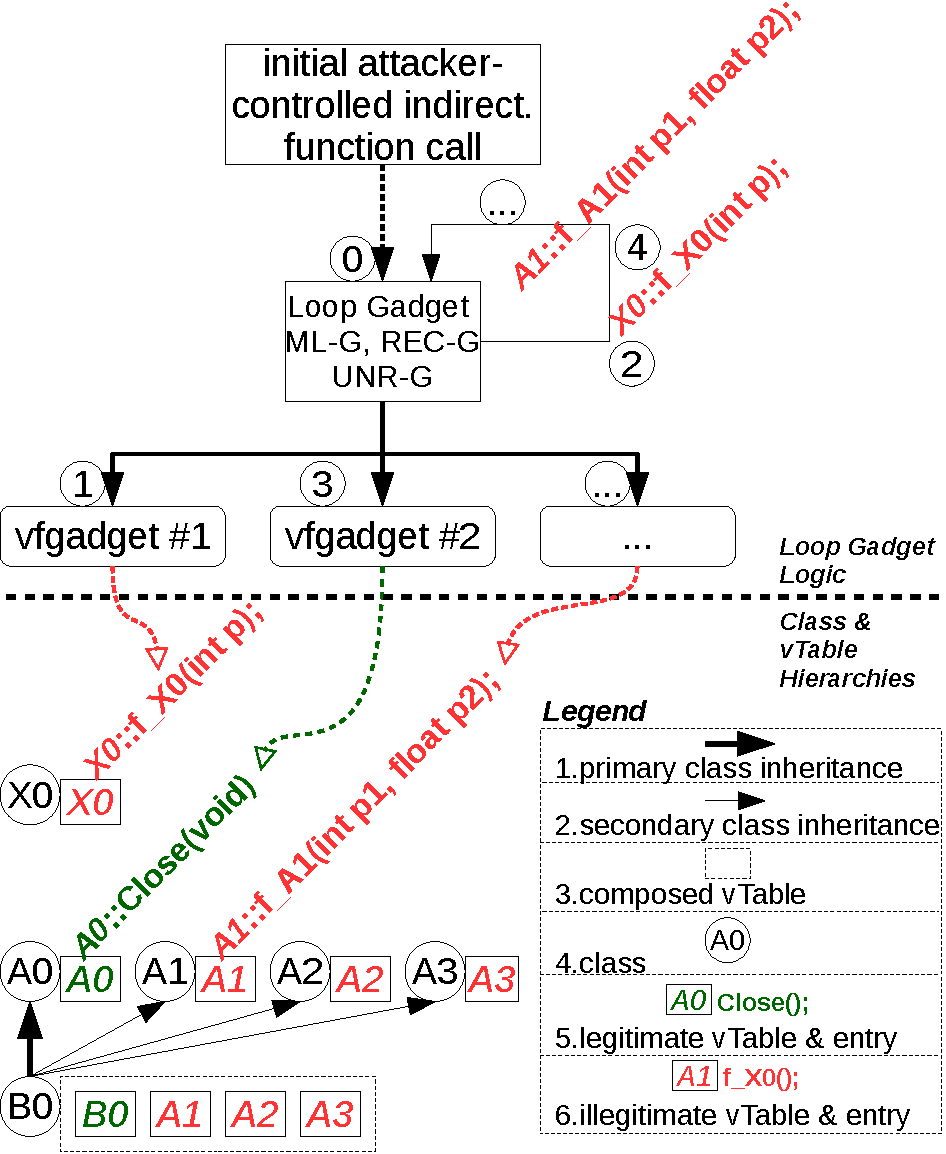
\includegraphics[width=1.3\textwidth]{figures/loop.pdf}
% \end{minipage}
% \caption{Code example used to illustrate how a COOP loop gadget works.}
% \label{Code example used to illustrate how a COOP loop gadget works}
% \end{figure}

%%%%%%%%%%%%%%%%%
%  \begin{figure*}[!t]
%     \centering
%    \setlength{\unitlength}{0.1\textwidth}
%    \begin{picture}(10,4)
% %    \centering
%      \put(4.81,0){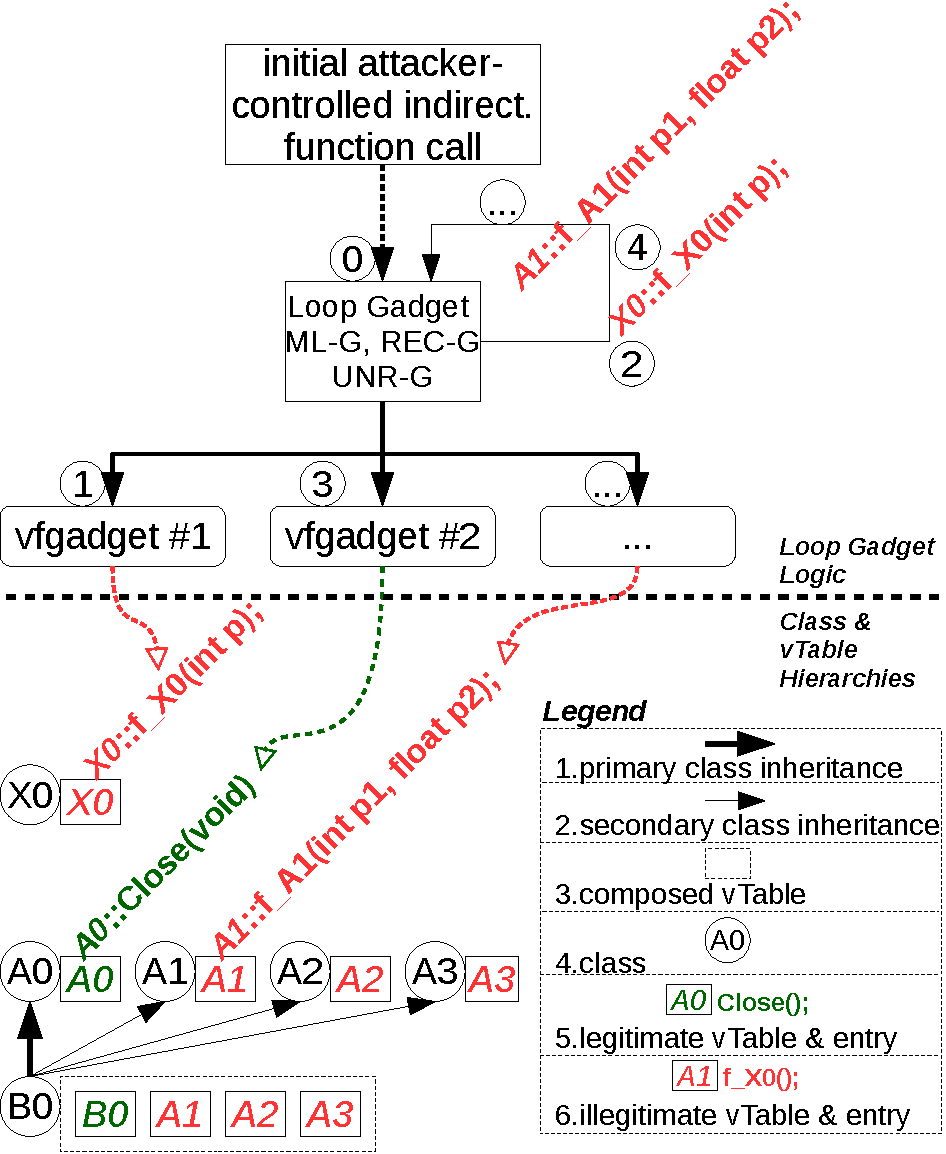
\includegraphics[width=.43\textwidth]{figures/loop.pdf}}
%      \put(1.5,2){\usebox{\firstlisting}}
%    \end{picture}
% \caption{Description of how a counterfeit object-oriented programming main loop gadget (ML-G) works.}
% \label{Code example used to illustrate how a COOP loop gadget works}
% \end{figure*}

%most probably not needed at this time.
% \label{Outline}
% \textbf{Outline.} 
% The remainder of this paper is organized as follows.
% \cref{C++ Bad Forward Indirect Calls} explains forbidden forward indirect calls issues and their security implications, and 
% \cref{chapter:TypeShild Overview} contains an overview of \textsc{TypeShield}.
% \cref{chapter:Design} describes the theory used and decisions made during the design of \textsc{TypeShield}, and
% \cref{chapter:Implementation} briefly presents the implementation details of \textsc{TypeShield}, while
% \cref{chapter:Evaluation} evaluates several properties of \textsc{TypeShield}.
% \cref{chapter:Discussion} contains the discussion, and
% \cref{chapter:Related_Work} surveys related work, while
% \cref{chapter:Future_Work} highlights future research venues. 
% Finally, \cref{chapter:Conclusion} concludes this paper.


